\chapter{The Encoding}
\label{ch:09}



\begin{center}
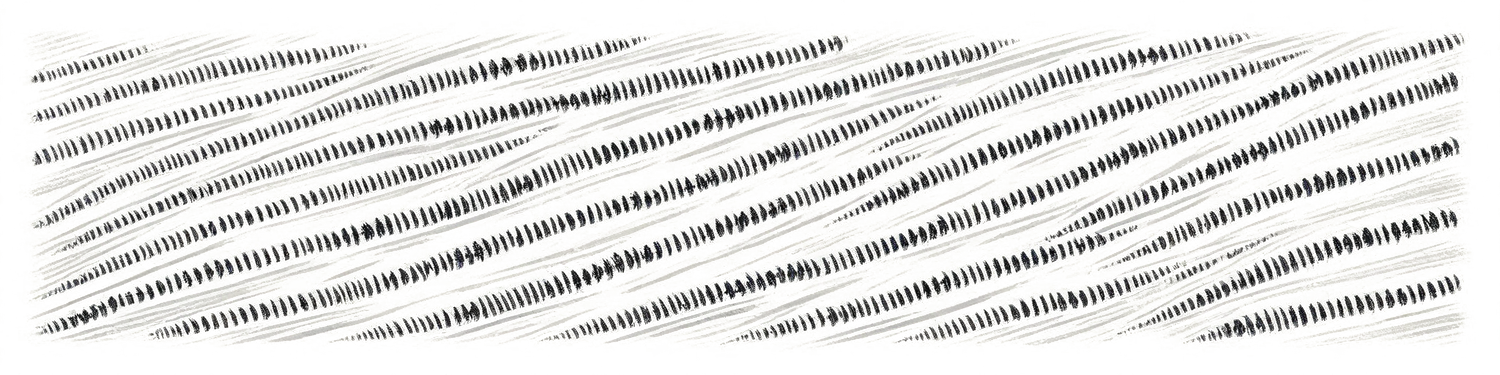
\includegraphics[width=\textwidth]{images/chapterImages/genesis_sketch_00077_.png}
\end{center}

The pattern was complete.

Not finished—it would never truly be finished, could always be refined, could always incorporate more detail. But complete in the sense that all necessary information had been encoded. All critical thresholds marked. All activation timelines established. All probability calculations rendered in stone and space and geometric relationship.

Aurelia stood at the pattern's center and looked at what had been created. Years of work. Thousands of stones. Every piece positioned with mathematical precision. The entire thing functioned as a map, a guide, a set of instructions for creating technological civilization from small mammals across 65 million years.

If it could be read. If anyone survived to read it. If the right minds emerged to interpret geometric relationships as information rather than random scatter.

If. Still always if.

But the work was complete.

879 rotations remaining.

\scenebreak

Around the pattern, the mammals lived their protected lives. The tool-using population had reached stable equilibrium—eighty-seven individuals. Tool use was culturally transmitted. Enhanced cognitive capability was breeding true. Some individuals showed fire-watching behavior. The thresholds were being crossed on schedule.

The tree-dwellers had developed complex social structures. Hierarchies based not just on strength but on problem-solving ability. The clever ones gained status. Gained more breeding opportunities. Intelligence selecting for itself in feedback loop that would amplify across generations.

Other mammal lineages showed different developments. Some had enhanced memory. Others showed better vocal control—the foundation for eventual language. Others showed increased manual dexterity beyond what their ecology strictly required. All selected traits. All guided evolution.

Aurelia had marked each lineage's territory with stones. Not the complex patterns of the main work. Simple markers. Designations. This population carries tool-use genes. This population carries social-complexity genes. This population carries vocal-control genes. When they merged—if they merged—if they survived to merge—the combination of traits would create something greater than any individual lineage.

The markers were arranged geographically to maximize survival probability while maintaining population separation. Distance enough to allow independent evolution. Proximity enough to enable eventual interbreeding once populations grew and ranges expanded.

She had calculated the optimal distribution. Had moved certain mammal populations by capturing and relocating individuals. Transported them in her mouth like prey, carried them miles from their original territories, released them in locations that the mathematics said offered better survival probability and better eventual merger dynamics.

The mammals didn't understand they were being positioned like pieces on a vast board. Didn't know their territories were being optimized. They simply adapted to new locations, bred, continued the cognitive development that had been selected for.

Each population: a different cluster in the pattern. Each cluster marked with specific stones that encoded the genetic modifications that population carried. The entire landscape had become a vast genetic map, readable if one understood the grammar.

\scenebreak

The daughter had completed her own pattern. Smaller than the Watcher's but sound in its mathematics. It focused on a specific section of the larger problem: atmospheric recovery post-impact. Carbon cycle. Oxygen levels. Temperature regulation. Climate return to pre-impact norms over tens of thousands of years.

Her pattern intersected with the Watcher's at key points. Supporting data. Complementary calculations. Two minds working the same problem from different angles, the results reinforcing each other.

The males had contributed their own sections. One focused on ocean recovery—the marine ecosystems would be devastated by impact, but some life would persist in deep waters. That life would reseed the oceans eventually. Understanding that timeline was critical for understanding when coastal populations of evolved mammals could utilize marine resources. When seafaring would become possible. When global connectivity would enable the final technological acceleration.

The other male focused on geological processes. Mineral access. Where certain elements critical for tool-making would be exposed by impact crater formation. Where volcanic activity would resurface useful materials. Where erosion would reveal what needed to be found when the time came.

All of it integrated into the master pattern. All of it connected through mathematical relationship. The scope was staggering. The precision required was impossible. They had achieved it anyway.

Other contributors had added their pieces across the continent. The Builder's pattern focused on the timeline itself—the step-by-step progression from one threshold to the next. Tool use to fire to agriculture to settlements to specialization to writing to mathematics to astronomy to physics to planetary defense. Each step necessary. Each step building on the previous. No shortcuts possible.

The cliff carvings detailed the genetic sequences. Which genes controlled brain size. Which controlled hand dexterity. Which controlled vocal apparatus. Which controlled social bonding. How to select for each. How to combine them. How to create a genome that would support technological civilization.

The patterns didn't contain the genes themselves—that was encoded differently, in the actual genetic material of the living mammals. But the cliff carvings mapped the genome. Explained which sequences mattered. Provided the instruction manual for reading what had been written into living flesh.

\scenebreak

The wrongstar had developed its tail. A bright streak across the sky. Beautiful if one didn't understand what it meant. Terrifying if one did.

Everyone understood.

Across the planet, the work had reached feverish completion. Not panic. Not desperation. Just the recognition that time was finite and the work needed finishing. Every individual capable of contribution contributed. Every mind that could calculate did calculate.

And then, gradually, the work stopped.

Not because it was complete—it could never be truly complete. But because there were no more stones to place. No more cliffs to carve. No more patterns to encode. The information that could be conveyed through physical positioning and geometric relationship had been conveyed. The rest would have to be carried in living flesh. In selected genes. In behavioral instinct encoded so deep that it would persist through 65 million years of evolution.

Aurelia stood in her pattern and waited for the mammals to emerge for evening foraging. They came on schedule. The tool-user led her family group. They foraged efficiently, using tools to access food sources. They shared food with offspring, teaching technique. They demonstrated problem-solving, social cohesion, forward planning.

She watched them with the same intensity she had watched the first tool-user years ago. But now she wasn't observing for new information. She was confirming that the traits had stabilized. That the modifications were complete. That what she had built into them would persist.

The tool-user noticed her watching. Paused in its foraging. They looked at each other across ten body lengths of space. Predator and prey. Creator and creation. Past and future.

The mammal didn't understand what it was. What it carried. What it would become.

Aurelia understood completely.

She made a soft sound. Not aggressive. Not possessive. Just... acknowledgment. The mammal had served its purpose. Had been shaped for a reason. Would carry forward the encoded potential even if it never knew why.

The mammal returned to foraging. Its family followed. They disappeared into the undergrowth.

She didn't follow. Didn't hunt. Just watched them go and ran calculations one more time. Survival probability for that specific lineage: 47\%. Higher than most. The tree-dwellers had 38\%. The social-complexity lineage had 52\%. The vocal-control group had 31\%.

Combined survival probability—at least one lineage persisting through impact winter: 89\%.

Probability that survivors retained the encoded traits: 71\%.

Probability that traits would propagate and amplify over time: 64\%.

Probability that technological civilization would emerge: 23\%.

Probability that civilization would achieve planetary defense before the next major impact: 8\%.

Eight percent.

She had spent years of her life, sacrificed everything that wasn't this work, driven herself and others to the edge of capability. Had calculated across timescales that turned individuals into statistical noise. Had encoded a plan so vast and complex that its mere existence was improbable.

For eight percent.

Eight percent wasn't good. Wasn't remotely sufficient. In any sane framework, eight percent was failure probability masquerading as success chance.

But it was better than zero. Better than extinction guarantee. Better than nothing persisting. Better than the wrongstar hitting an unprotected world and that being the end of possibility forever.

Eight percent was what mathematics and effort and sacrifice could purchase. And so it would have to be enough.

\scenebreak

That evening, the entire family gathered in the territory. The daughter with her mate and hatchlings. The males with their mates. The neighbor pairs who had been working on adjacent patterns. A dozen individuals total. Three generations. All still living to see the project completed.

They didn't gather for ceremony. Their kind didn't do ceremony. But they gathered anyway, drawn by some shared recognition that the work phase had ended. That what came next was different. Was waiting. Was the helpless time when all variables were locked and all calculations were complete and nothing remained but to observe outcome.

They stood in loose formation around the pattern's central section. The master plan. The encoded timeline. The mathematical proof that survival was possible.

The wrongstar rose bright enough to read by. Bright enough to cast shadows. Bright enough that nocturnal creatures were becoming confused, sometimes treating night as day.

No one moved. No one calculated. No one worked. They simply stood together and watched the sky and waited for what would come.

A young one—one of the daughter's hatchlings—broke the silence with a questioning chirp. Too young to understand. Too young to feel the weight of what approached. It was shushed gently by its parent.

Aurelia looked at that young one. Calculated its age. It would be adolescent at impact. Old enough to hunt independently. Young enough that it might survive on less food during the resource-scarce years. Its survival probability was actually slightly higher than the adults'. Small size advantage. Lower caloric requirements. Better hide-and-wait capability.

If it survived, if it bred after the impact, if it passed on any fragment of knowledge...

But that was speculation beyond the scope of current planning. The encoding was complete. The dice were cast. The wrongstar approached on its inevitable trajectory.

836 rotations remaining.

\scenebreak

Over the following weeks, the pattern became... something else. Not abandoned. Not forgotten. But no longer actively worked. It simply existed. A monument to effort. A message to the future. A plan that would either unfold or fail to unfold across time scales beyond imagining.

Life continued around it. The mammals foraged and bred and raised young. The dinosaurs hunted and protected and maintained the selective pressures that shaped the mammal populations. But the feverish intensity was gone. The desperate push toward completion had completed. What remained was maintenance. Waiting. The patient countdown toward event horizon.

Aurelia spent less time at the pattern. More time in simple observation. Watching the mammals. Watching the sky. Watching her family and the neighbors and the whole community of calculation that had emerged around the project.

She hunted more. Needed to rebuild reserves depleted by months of minimal intake. Her body had suffered from the sustained effort. She was thinner than healthy. Her feathers showed damage. She needed recovery time.

But there was recovery time now. 800-some rotations was plenty for physical restoration. The work didn't require her attention anymore. The pattern was stable. The mammals were successfully breeding. The plan was encoded and waiting for its unimaginably distant activation.

She could rest.

She stood sometimes at the marked stone where the other one had been. The grass had grown tall around it. Small flowers bloomed in season. Life continued. Matter cycled. The world persisted in its patterns.

She wondered if he had understood the full scope. If his mathematics had reached far enough forward to comprehend what they were attempting. Or if he had simply contributed what he could calculate and trusted that it connected to something larger.

She would never know. His calculations had terminated. Her calculations continued. And the pattern that incorporated his work would either succeed or fail independent of either of them.

That was the nature of deep time planning. No one would know if it worked. Success would occur so far in the future that it might as well be in a different universe. Causality stretched so thin across 65 million years that the connection between action now and result then became almost metaphysical.

But the mathematics was sound. The encoding was complete. And eight percent was better than zero.

She looked at the wrongstar—now bright enough that it hurt to look directly at it. Developing structure. The tail streaming behind. The signature of terminal approach.

Soon. Very soon now.

The waiting was almost over.

